\chapter{Hyperparameters and Model Validation\label{Ch39}}
\section{Thinking About Model Validation}
In principle, model validation is very simple: after choosing a model and its hyperparameters, we can estimate how effective it is by applying it to some of the training
data and comparing the predictions to the known values.
\subsection*{Model Validation the Right Way: Holdout Sets}
A better sense of a model's performance can be found by using
what's known as a \textit{holdout set}: that is, we hold back some subset of the data from the
training of the model, and then use this holdout set to check the model's performance.
\subsection*{Model Validation via Cross-Validation}
One disadvantage of using a holdout set for model validation is that we have lost a
portion of our data to the model training.

One way to address this is to use cross-validation; that is, to do a sequence of fits
where each subset of the data is used both as a training set and as a validation set.

cikit-Learn implements a number of cross-validation schemes that are useful in particular situations; these are implemented via iterators in the \verb|model_selection| module. For example, we might wish to go to the extreme case in which our number of
folds is equal to the number of data points: that is, we train on all points but one in
each trial. This type of cross-validation is known as \textit{leave-one-out}\marginpar[留一验证]{留一验证} cross validation.

\section{Selecting the Best Model}
\subsection*{The Bias-Variance Trade-off}
Fundamentally, finding “the best model” is about finding a sweet spot in the trade-off
between bias and variance.

欠拟合的模型会有较高的偏差(bias),过拟合的模型甚至拟合了数据中的随机误差,这样的模型具有较高的方差(variance)。

The $R^2$ score, or coefficient of determination, measures how
well a model performs relative to a simple mean of the target values. $R^2 = 1$ indicates
a perfect match, $R^2 = 0$ indicates the model does no better than simply taking the
mean of the data, and \important{negative values mean even worse models}.

If we imagine that we have some ability to tune the model complexity, we would
expect the training score and validation score to behave as illustrated in \autoref{fig39-5},
often called a validation curve, and we see the following features:
\begin{itemize}
      \item The training score is everywhere higher than the validation score. This is generally the case: the model will be a better fit to data it has seen than to data it has
            not seen.
      \item For very low model complexity (a high-bias model), the training data is underfit,
            which means that the model is a poor predictor both for the training data and for
            any previously unseen data.
      \item For very high model complexity (a high-variance model), the training data is
            overfit, which means that the model predicts the training data very well, but fails
            for any previously unseen data.
\end{itemize}

\begin{figure}
      \centering
      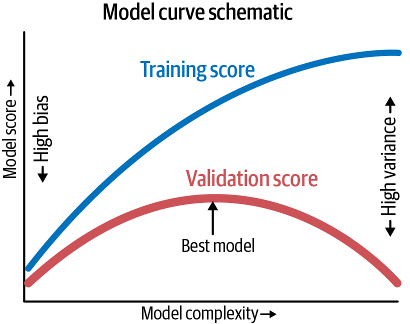
\includegraphics{../img/fig39-5.png}
      \caption{A schematic of the relationship between model complexity, training score, and validation score}
      \label{fig39-5}
\end{figure}

A useful question to answer is this: which model provides a suitable trade-off between bias (underfitting) and
variance (overfitting)?

We can make progress in this by visualizing the validation curve for this particular
data and model; this can be done straightforwardly using the \verb|validation_curve| convenience routine provided by Scikit-Learn. Given a model, data, parameter name,
and a range to explore, this function will automatically compute both the training
score and the validation score across the range.

\section{Learning Curves}
One important aspect of model complexity is that the optimal model will generally
depend on the size of your training data.

The behavior of the validation curve has not one but two important inputs: the
model complexity and the number of training points.

We can gain further insight by
exploring the behavior of the model as a function of the number of training points,
which we can do by using increasingly larger subsets of the data to fit our model. \important{A
      plot of the training/validation score with respect to the size of the training set is
      sometimes known as a \textit{learning curve}.}

The general behavior we would expect from a learning curve is this:
\begin{itemize}
      \item A model of a given complexity will overfit a small dataset: this means the training
            score will be relatively high, while the validation score will be relatively low.
      \item A model of a given complexity will underfit a large dataset: this means that the
            training score will decrease, but the validation score will increase.
      \item A model will never, except by chance, give a better score to the validation set than
            the training set: this means the curves should keep getting closer together but
            never cross.
\end{itemize}

With these features in mind, we would expect a learning curve to look qualitatively
like that shown in \autoref{fig39-11}.

\begin{figure}
      \centering
      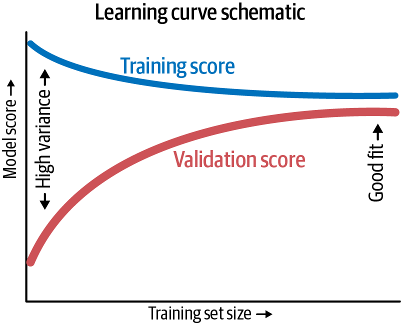
\includegraphics{../img/fig39-11.png}
      \caption{Schematic showing the typical interpretation of learning curves}
      \label{fig39-11}
\end{figure}

The notable feature of the learning curve is the convergence to a particular score as
the number of training samples grows. In particular, once you have enough points
that a particular model has converged, adding more training data will not help you!
The only way to increase model performance in this case is to use another (often
more complex) model.

\figures{Learning curves for a low-complexity model and a high-complexity model}

\autoref{Learning curves for a low-complexity model and a high-complexity model} is a valuable diagnostic, because it gives us a visual depiction of how our model
responds to increasing amounts of training data. In particular, when the learning
curve has already converged (i.e., when the training and validation curves are already
close to each other) adding more training data will not significantly improve the fit!
This situation is seen in the left panel, with the learning curve for the degree-2 model.

The only way to increase the converged score is to use a different (usually more complicated) model. We see this in the right panel: by moving to a much more complicated model, we increase the score of convergence (indicated by the dashed line), but
at the expense of higher model variance (indicated by the difference between the
training and validation scores). If we were to add even more data points, the learning
curve for the more complicated model would eventually converge.

Plotting a learning curve for your particular choice of model and dataset can help you
to make this type of decision about how to move forward in improving your analysis.

\section{Validation in Practice: Grid Search}
GridSearchCV include the ability to specify a custom scoring function, to parallelize the computations, to do randomized searches, and more.